\documentclass[10 pt,usenames,dvipsnames, oneside]{article}
\usepackage{../../../modelo-ensino-medio}



\begin{document}

\begin{center}
  \begin{minipage}[l]{3cm}

\includegraphics[width=2cm]{logo}    
\end{minipage}\hfill
\begin{minipage}[r]{.8\textwidth}
 {\Large \scshape Atividade: }  
\end{minipage}
\end{center}
\vspace{.2cm}

\ifdefined\prof
\begin{objetivos}
\item \textbf{EM13MAT401} Converter representações algébricas de funções polinomiais de 1º grau em representações geométricas no plano cartesiano, distinguindo os casos nos quais o comportamento é proporcional, recorrendo ou não a softwares ou aplicativos de álgebra e geometria dinâmica.
\item \textbf{EM13MAT507} Identificar e associar progressões aritméticas (PA) a funções afins de domínios discretos, para análise de propriedades, dedução de algumas fórmulas e resolução de problemas.
\end{objetivos}

\begin{goals}
\begin{enumerate}
\item Identificar a expressão algébrica que expressa a regularidade observada na sequência apresentada na figura.
\item Identificar funções de domínio discreto e observar a implicação na representação gráfica.
\end{enumerate}

\tcblower

\begin{itemize}
\item Nesta atividade o estudante deve identificar que o domínio de ambas as funções é um conjunto discreto e que esse fato tem implicações no gráfico das funções, que serão conjuntos de pontos colineares, mas não serão retas.
\item Ainda neste ano de escolaridade boa parte dos alunos terão dificuldades de identificar a expressão algébrica que expressa a relação entre as grandezas apresentadas na figura, caso essa dificuldade atrapalhe o andamento da atividade, sugerimos que o professor intervenha exibindo exemplos mais simples do mesmo assunto.
\item Aproveite para comentar com os alunos que as funções $C(n)$ descrita no item e) é uma função quadrática com domínio discreto, e que esse será o assunto de um capítulo envolvendo funções quadráticas.
\item A atividade aborda assuntos relacionados a dois temas transversais, tais como Meio Ambiente, Saúde e sustentabilidade. Sugerimos que procure fazer um trabalho colaborativo com os professores de Biologia e de Geografia para ampliar a discussão com os alunos sobre os benefícios de uma alimentação orgânica e sobre as questões de viabilidade econômica e de sustentabilidade de tal tipo de cultura. 

\end{itemize}

\end{goals}

\bigskip
\begin{center}
{\large \scshape Atividade}
\end{center}
\fi

No cultivo de produtos orgânicos, é comum o plantio de Plantas Companheiras. "Plantas Companheiras são plantas pertencentes a espécies ou famílias que se ajudam e complementam mutuamente, não apenas na ocupação do espaço e utilização de água, luz e nutrientes, mas também por meio de interações bioquímicas chamadas de Efeitos Alelopáticos. Estes podem ser tanto de natureza estimuladora quanto inibidora, não somente entre plantas, mas também em relação a insetos e outros animais." Disponível \href{https://permacoletivo.files.wordpress.com/2008/06/manual-horta-organica-domestica.pdf}{neste link} - Acesso em 25/11/2017.

Uma empresa especializada em consultoria e plantio de produtos orgânicos apresenta alguns modelos de plantio de um determinado vegetal, representado na figura a seguir por ({\Large $\bullet$}) e sua respectiva planta companheira ({\Large$\diamondsuit$}), cada modelo é adequado para o tamano do plantio e tem como objetivo criar uma barreira natural contra pragas, observe a figura a seguir que apresenta os modelos de plantio, identificados sequencialmente por Modelo 1, Modelo 2, Modelo 3, ..., Modelo $n$.


\begin{figure}[H]
\centering

\begin{tikzpicture}[node distance=10pt, every node/.style={scale=2.5}]

\begin{scope}[local bounding box=scope1]
\node (a1) {$\diamondsuit$};
\node (a2) [right of=a1] {$\diamondsuit$};
\node (a3) [above of=a2] {$\diamondsuit$};
\node (a4) [above of=a1] { $\diamondsuit$};

\node (b) [yshift=5pt] at ($(a1)!.5!(a2)$) { $\bullet$};

\node (c) at ($(a1)!.5!(a2)$) {};

\node [below of=c, scale=.5] {Modelo 1};

\end{scope}

\begin{scope}[xshift=70]
\node (a1) {$\diamondsuit$};
\node (a2) [right of=a1] {$\diamondsuit$};
\node (a3) [right of=a2] {$\diamondsuit$};

\node (a4) [above of=a1] {$\diamondsuit$};
\node (a5) [above of=a4] {$\diamondsuit$};
\node (a6) [right of=a5] {$\diamondsuit$};
\node (a7) [right of=a6] {$\diamondsuit$};
\node (a8) [above of=a3] {$\diamondsuit$};

\node (b1) [yshift=5pt] at ($(a1)!.5!(a2)$) { $\bullet$};
\node (b2) [right of=b1] {$\bullet$};
\node (b3) [above of=b1] {$\bullet$};
\node (b4) [above of=b2] {$\bullet$};

\node [below of=a2, scale=.5] {Modelo 2};
\end{scope}

\begin{scope}[xshift=170]
\node (a1) {$\diamondsuit$};
\node (a2) [right of=a1] {$\diamondsuit$};
\node (a3) [right of=a2] {$\diamondsuit$};
\node (a4) [right of=a3] {$\diamondsuit$};

\node (a5) [above of=a1] {$\diamondsuit$};
\node (a6) [above of=a5] {$\diamondsuit$};
\node (a7) [above of=a6] {$\diamondsuit$};
\node (a8) [right of=a7] {$\diamondsuit$};
\node (a9) [right of=a8] {$\diamondsuit$};
\node (a10) [right of=a9] {$\diamondsuit$};
\node (a11) [above of=a4] {$\diamondsuit$};
\node (a12) [above of=a11] {$\diamondsuit$};


\node (b1) [yshift=5pt] at ($(a1)!.5!(a2)$) { $\bullet$};
\node (b2) [right of=b1] {$\bullet$};
\node (b3) [right of=b2] {$\bullet$};

\node (b4) [above of=b1] {$\bullet$};
\node (b5) [above of=b4] {$\bullet$};
\node (b6) [right of=b5] {$\bullet$};
\node (b7) [right of=b6] {$\bullet$};
\node (b8) [above of=b3] {$\bullet$};
\node (b9) [above of=b2] {$\bullet$};

\node (c) at ($(a2)!.5!(a3)$) {};

\node [below of=c, scale=.5] {Modelo 3};
\end{scope}

\begin{scope}[xshift=300]
\node (a1) {$\diamondsuit$};
\node (a2) [right of=a1] {$\diamondsuit$};
\node (a3) [right of=a2] {$\diamondsuit$};
\node (a4) [right of=a3] {$\diamondsuit$};
\node (a5) [right of=a4] {$\diamondsuit$};

\node (a6) [above of=a1] {$\diamondsuit$};
\node (a7) [above of=a6] {$\diamondsuit$};
\node (a8) [above of=a7] {$\diamondsuit$};
\node (a9) [above of=a8] {$\diamondsuit$};

\node (a10) [right of=a9] {$\diamondsuit$};
\node (a11) [right of=a10] {$\diamondsuit$};
\node (a12) [right of=a11] {$\diamondsuit$};
\node (a13) [right of=a12] {$\diamondsuit$};

\node (a14) [above of=a5] {$\diamondsuit$};
\node (a15) [above of=a14] {$\diamondsuit$};
\node (a16) [above of=a15] {$\diamondsuit$};
\node (a17) [above of=a16] {$\diamondsuit$};


\node (b1) [yshift=5pt] at ($(a1)!.5!(a2)$) { $\bullet$};
\node (b2) [right of=b1] {$\bullet$};
\node (b3) [right of=b2] {$\bullet$};
\node (b4) [right of=b3] {$\bullet$};

\node (b5) [above of=b1] {$\bullet$};
\node (b6) [above of=b5] {$\bullet$};
\node (b7) [above of=b6] {$\bullet$};
\node (b8) [right of=b7] {$\bullet$};
\node (b9) [right of=b8] {$\bullet$};
\node (b10) [right of=b9] {$\bullet$};
\node (b11) [above of=b4] {$\bullet$};
\node (b12) [above of=b11] {$\bullet$};

\node (b13) [right of=b5] {$\bullet$};
\node (b14) [right of=b13] {$\bullet$};
\node (b15) [right of=b14] {$\bullet$};

\node (b16) [right of=b6] {$\bullet$};
\node (b17) [right of=b16] {$\bullet$};
\node (b18) [right of=b17] {$\bullet$};

\node [below of=a3, scale=.5] {Modelo 4};
\end{scope}

\end{tikzpicture}
\end{figure}

\begin{enumerate}
\item Preencha o quadro a seguir, que nos informa a quantidade de cada tipo de planta em cada um dos modelos.

\begin{table}[H]
\centering
\setlength\tabulinesep{2.5pt}
\begin{tabu} to \textwidth{|l|>{\centering}m{2cm}|>{\centering}m{2cm}|}
\hline
& ({\Large$\bullet$}) & ({\Large$\diamondsuit$}) \\
\hline
Modelo 1 & & \\
\hline
Modelo 2 & & \\
\hline
Modelo 3 & & \\
\hline
Modelo 4 & & \\
\hline
\end{tabu}
\end{table}
\item Descreva textualmente qual a relação entre a quatidade de vegetais ({\Large$\bullet$}) e o número $n$ que identifica o modelo na sequência.

\item Descreva textualmente qual a relação entre a quantidade de plantas companheiras ({\Large$\diamondsuit$}) e o número $n$ que identifica o modelo na sequência.
\item Exiba uma expressão algébrica que relacione a quantidade $V$ de vegetais ({\Large$\bullet$}) em função do número $n$ que identifica o $n$-ésimo modelo na sequência.
\item xiba uma expressão algébrica que relacione a quantidade $V$ de vegetais ({\Large$\diamondsuit$}) em função do número $n$ que identifica o $n$-ésimo modelo na sequência.
\item No plano cartesiano a seguir estão representados os pares ordenados $(n,V(n))$ em que $n$ é o "número"{} que representa o $n$-ésimo modelo e $V(n)$ a quantidade $V$ de vegetais ({\Large$\bullet$}). Represente nele os pontos que correspondem aos pares ordenados $(n,C(n0)$ em que $C(n)$ é a quantidade $C$ de plantas companheiras ({\Large$\diamondsuit$}) em função de $n$.

\begin{figure}[H]
\centering
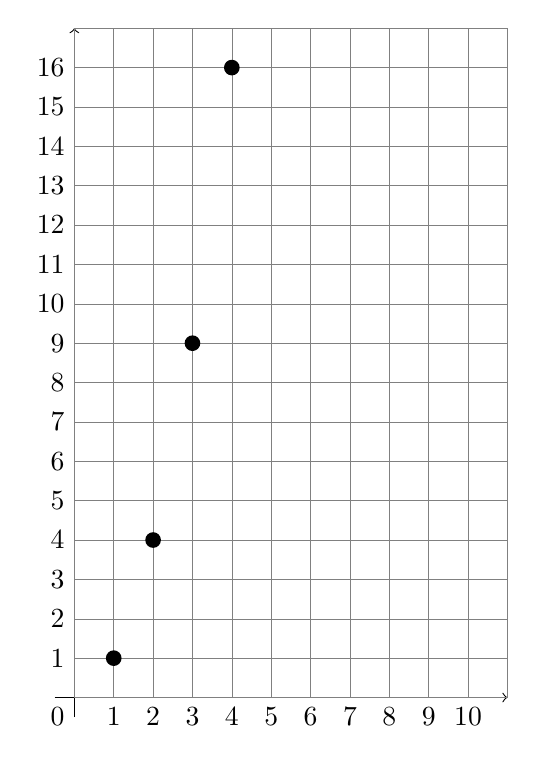
\begin{tikzpicture}[scale=.5]
\draw [->] (-.5,0) -- (11,0);
\draw [->] (0,-.5) -- (0,17);
\draw [help lines] (0,0) grid (11,17);

\foreach \x in {1,...,10} \node [below] at (\x,0) {\x};
\foreach \x in {1,...,16} \node [left] at (0,\x) {\x};
\node [below left] {0};

\foreach \x/\y in {1/1, 2/4, 3/9, 4/16} \node [fill, circle, inner sep=2pt] at (\x,\y) {};

\end{tikzpicture}

\end{figure}
\item Qual a quantidade $C$ de plantas companheiras ({\Large$\diamondsuit$}) utilizadas no décimo modelo?
\item Qual o valor de $n$ para um modelo que utilize $144$ plantas companheiras ({\Large$\diamondsuit$})?
\end{enumerate}


\ifdefined\prof
\begin{solucao}
\begin{enumerate}
\item \adjustbox{valign=t}
{
\setlength\tabulinesep{2.5pt}
\begin{tabu} to \textwidth{|l|>{\centering}m{2cm}|>{\centering}m{2cm}|}
\hline

& ({\Large$\bullet$}) & ({\Large$\diamondsuit$}) \\
\hline
Modelo 1 & 1 & 4 \\
\hline
Modelo 2 & 4 & 8 \\
\hline
Modelo 3 & 9 & 12 \\
\hline
Modelo 4 & 16 & 16 \\
\hline
\end{tabu}
}

\item A quantidade de vegetais ({\Large$\bullet$}) é o quadrado do número $n$ que identifica a ordem do modelo na sequência

\item A quantidade de plantas companheiras ({\Large$\diamondsuit$}) é o quádruplo do número do modelo.

\item $V(n)=n^2$

\item $C(n)=4n$
\clearpage
\item \adjustbox{valign=t}
{
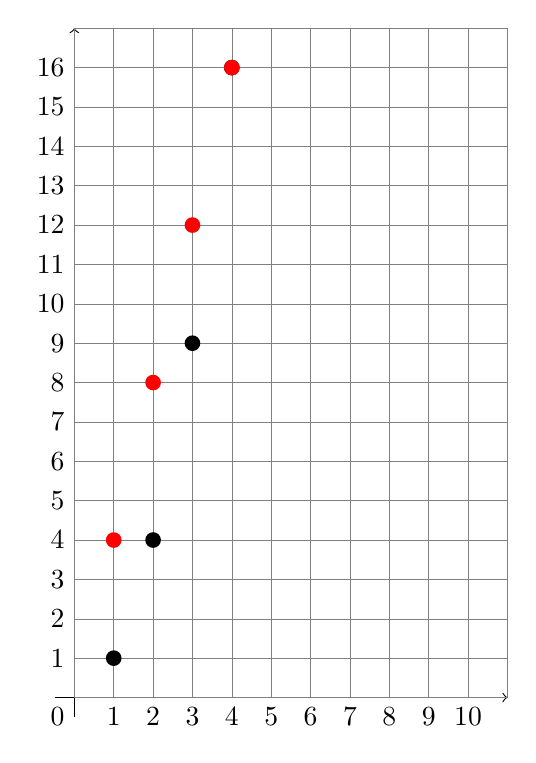
\begin{tikzpicture}[scale=.5]
\draw [->] (-.5,0) -- (11,0);
\draw [->] (0,-.5) -- (0,17);
\draw [help lines] (0,0) grid (11,17);

\foreach \x in {1,...,10} \node [below] at (\x,0) {\x};
\foreach \x in {1,...,16} \node [left] at (0,\x) {\x};
\node [below left] {0};

\foreach \x/\y in {1/1, 2/4, 3/9, 4/16} \node [fill, circle, inner sep=2pt] at (\x,\y) {};

\foreach \x/\y in {1/4, 2/8, 3/12, 4/16} \node [fill, circle, inner sep=2pt, red] at (\x,\y) {};

\end{tikzpicture}
}

\item $C(10)=40$

\item 36
\end{enumerate}
\end{solucao}
\fi

\end{document}